\documentclass[border=3pt,tikz]{standalone}
\usepackage{amsmath}
\begin{document}
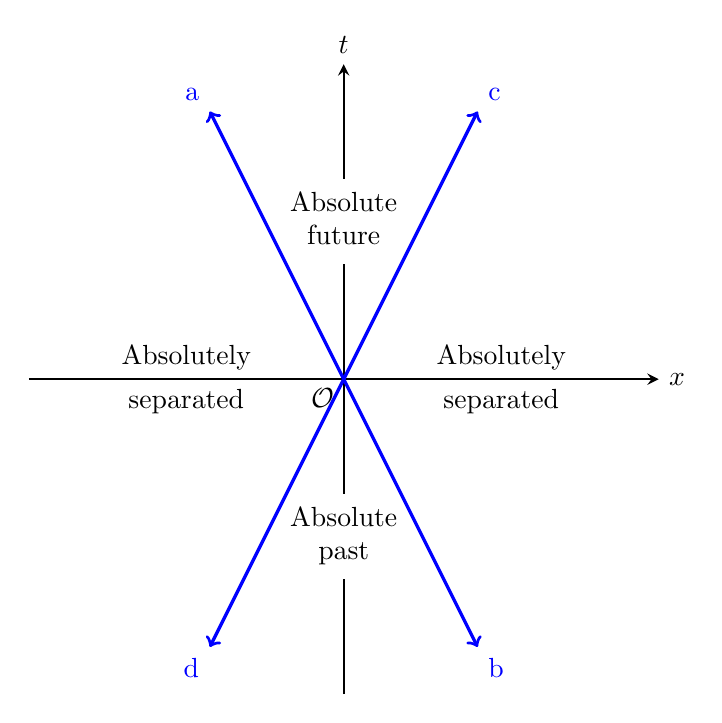
\begin{tikzpicture}[]
    \draw[thick,->,>=stealth] (0, -4) -- (0, 4) node[above] {$t$};
    \draw[thick,->,>=stealth] (-4, 0) -- (4, 0) node[right] {$x$};
    \node[below left] at (0, 0) {$\mathcal{O}$};
    \node[fill=white] at (0, 2) {\begin{tabular}{c} Absolute \\ future \end{tabular}};
    \node[fill=white] at (0, -2) {\begin{tabular}{c} Absolute \\ past \end{tabular}};
    \draw[very thick, blue, ->] (0,0)-- (1.7, 3.4) node[above right] {c};
    \draw[very thick, blue, ->] (0,0)-- (-1.7, 3.4) node[above left] {a};
    \draw[very thick, blue, ->] (0,0)-- (-1.7, -3.4) node[below left] {d};
    \draw[very thick, blue, ->] (0,0)-- (1.7, -3.4) node[below right] {b};

    \node[above] at (-2, 0) {Absolutely};
    \node[below] at (-2, 0) {separated};
    \node[above] at (2, 0) {Absolutely};
    \node[below] at (2, 0) {separated};

    \end{tikzpicture}

\end{document}